\section{PCB-ontwerp}
Voor het ontwerp van de custom Arduino PCB hebben we gewerkt met Eagle. Vertrekkende van de offici\"{e}le schematic van de Arduino Uno maken we onze eigen versie hiervan. Na de ontwerpfase kunnen we de PCB etsen, boren, bestukken en solderen. Als dit allemaal achter de rug is, testen we onze custom Arduino en lossen we nog eventuele problemen op. 
\subsection{Eagle-ontwerp}
\subsubsection{Schematic}
Om te beginnen hebben we het offici\"{e}le schema nodig van de Arduino Uno, welke makkelijk online te vinden is (zie figuur~\vref{fig:ardsch}). Om te weten wat we effectief nodig hebben en wat weggelaten mag worden, bestuderen we het schema grondig. Hierdoor zien we in dat er veel weg kan vallen uit het originele ontwerp, zoals de USB to serial interface. Aangezien we beslissen om onze custom Arduino te programmeren via de ICSP-pinnen, is de aanwezigheid van een USB-connectie overbodig. Dit zorgt ervoor dat de ATMEGA16U2 chip en al zijn connecties niet nodig zijn op onze eigen PCB. Ook onze voedingslijn wordt hierdoor minder complex: we hoeven ons geen zorgen te maken om de batterijspanning af te koppelen eens we een USB-connectie zouden gebruiken van onze computer. Vervolgens zijn ook alle LED's uit het offici\"{e}le ontwerp gehaald, zodat nog een IC (die twee opamps bevat), enkele weerstanden en een ontkoppelcondensator kunnen weggelaten worden. Ten slotte integreren we de Arduino Motorshield in ons ontwerp. De hoofdcomponent van dit gedeelte bestaat uit de L298P dual full-bridge driver en bevat de nodige afschermdiodes voor de motor outputs. Het resultaat is onze vereenvoudigde versie van de Arduino Uno (zie figuur~\vref{fig:eigensch}) dat we vervolgens kunnen gaan boarden.

\begin{figure}[H]
	\centering
	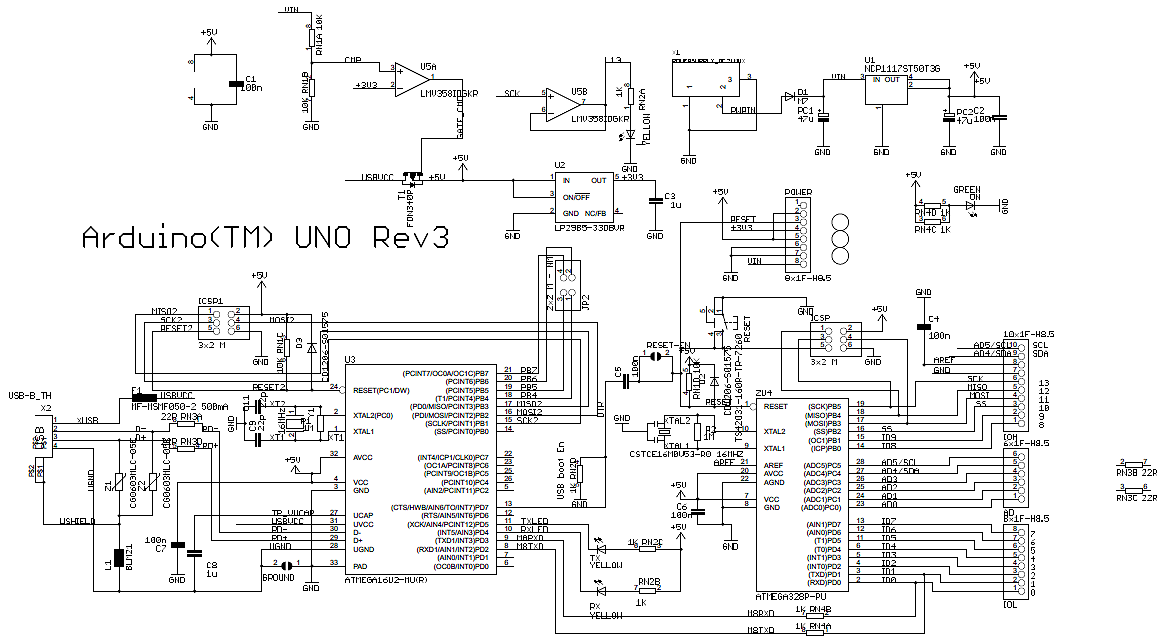
\includegraphics[width=\textwidth]{arduino-uno-r3-schematic.png}
	\caption{Offici\"{e}le schema van de Arduino Uno\label{fig:ardsch}}
\end{figure}

\begin{figure}[H]
	\centering
	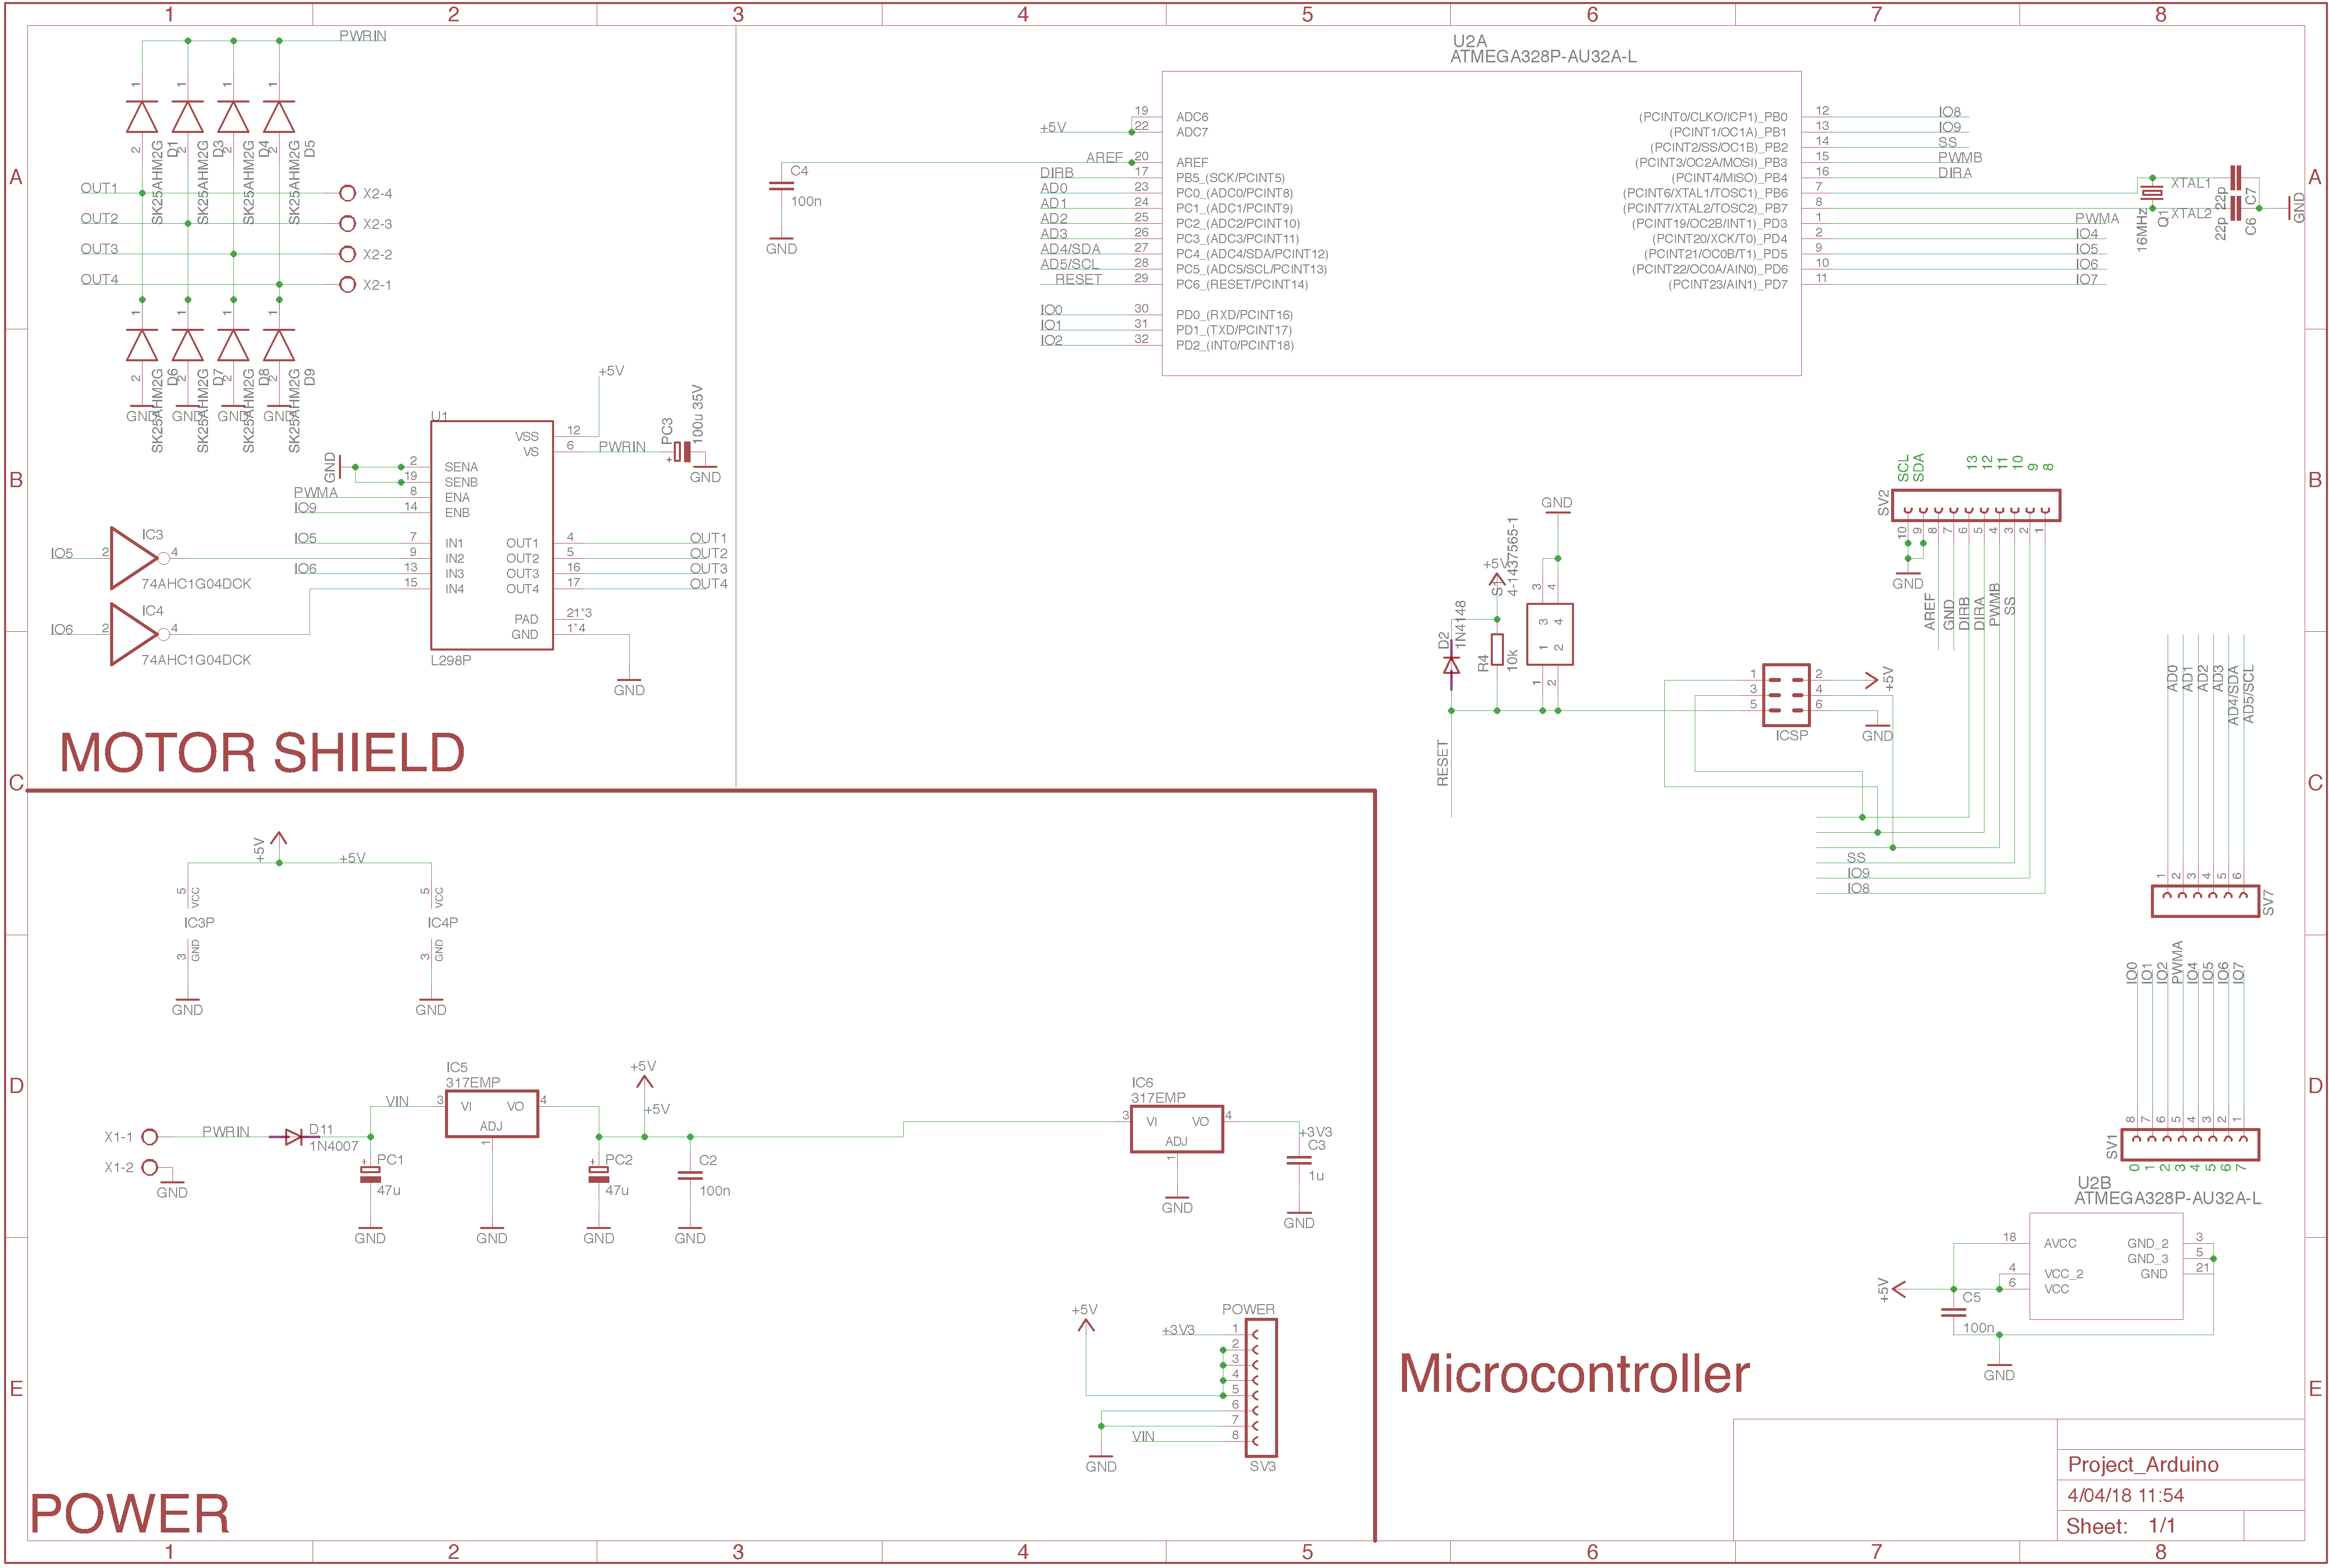
\includegraphics[width=\textwidth]{eigenschematic.png}
	\caption{Eigen schema van de Arduino Uno\label{fig:eigensch}}
\end{figure}

\subsubsection{Board}
Nu onze eigen schematic afgerond is, kunnen we beginnen boarden. We trachtten de PCB zo klein mogelijk te maken door de componenten zowel op de top- als de bottom-layer te plaatsen. We hebben ervoor gekozen de twee chips (de ATMEGA328P en de L298P) op de bottom-layer te plaatsen samen met de de nodige ontkoppelcondensatoren. De andere componenten staan op de top-layer. Na het routing proces bestaat onze PCB uit 20 via's. We hebben ook een massa vlak voorzien aan de bovenkant. De top- en bottom-layer van de PCB kan u vinden in respectievelijk figuur~\vref{fig:topboard} en figuur~\vref{fig:bottomboard}.

\begin{figure}[H]
	\centering
	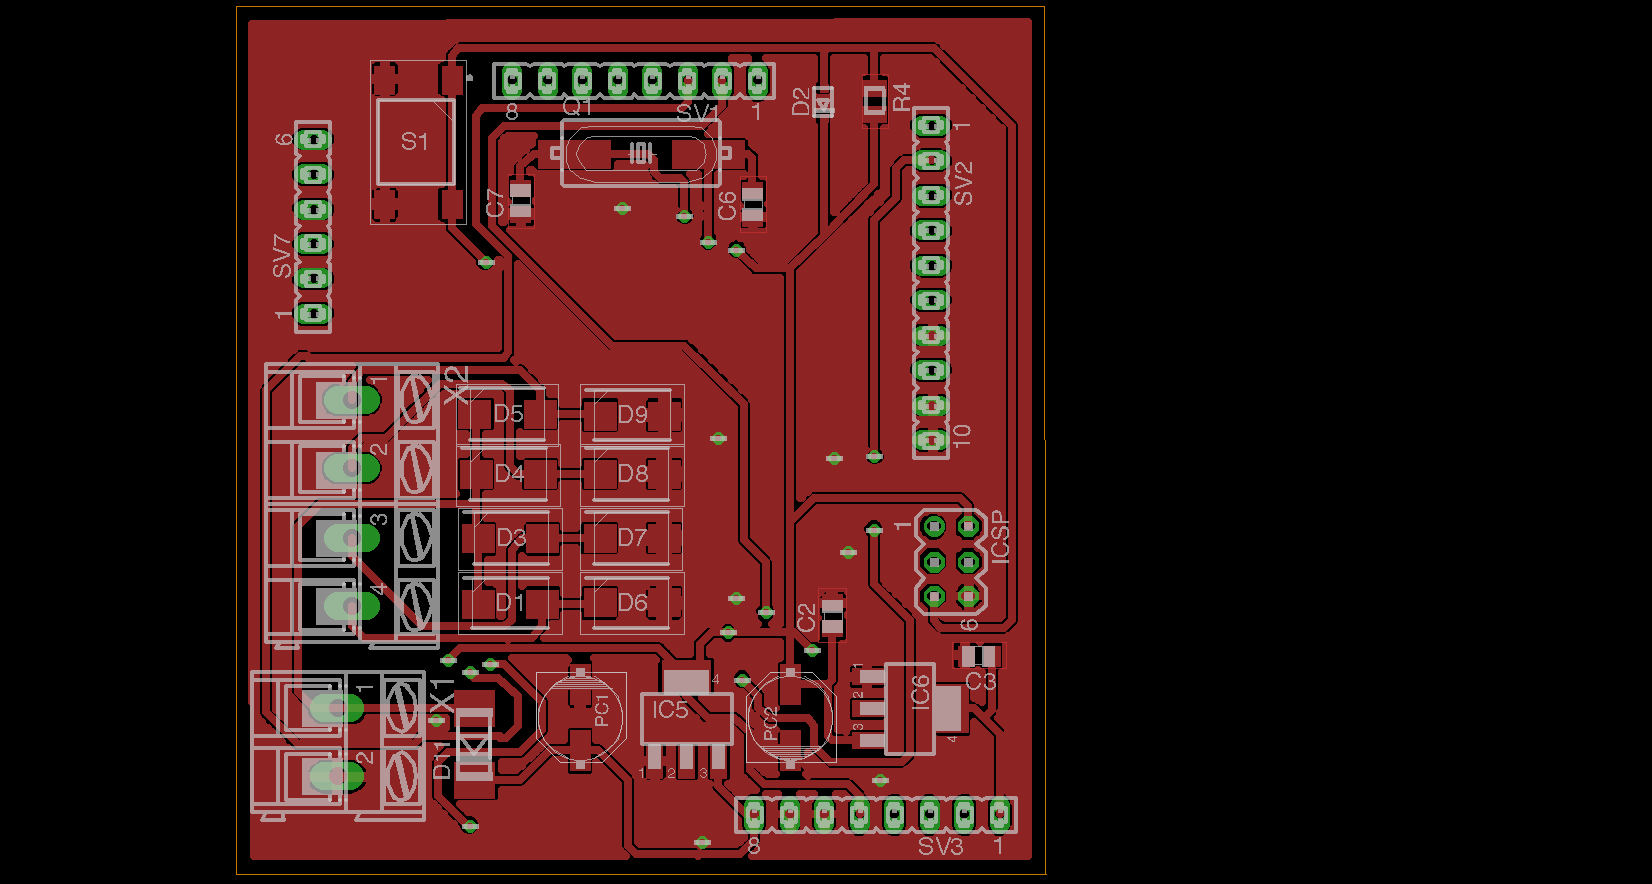
\includegraphics[height=5cm]{topboard.png}
	\caption{Eigen board van de Arduino Uno\label{fig:topboard}}
\end{figure}

\begin{figure}[H]
	\centering
	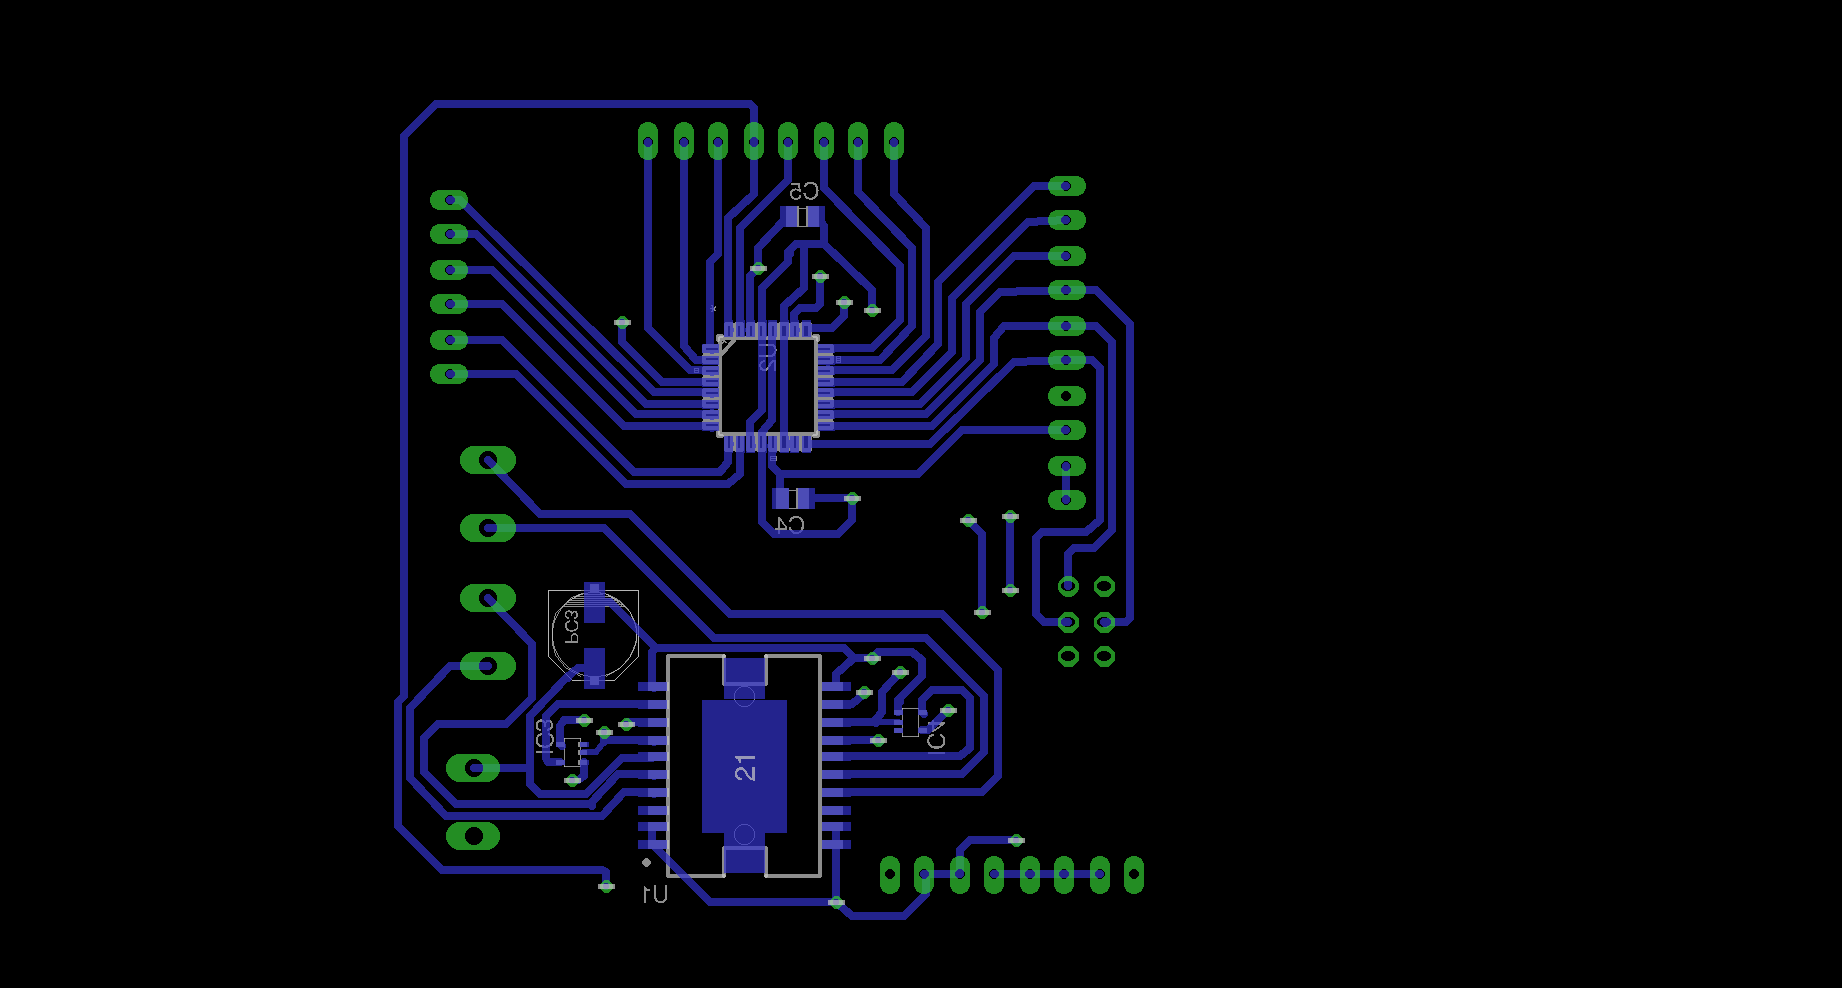
\includegraphics[height=5cm]{bottomboard.png}
	\caption{Eigen board van de Arduino Uno\label{fig:bottomboard}}
\end{figure}
\subsection{Maken van de PCB}
Het ontwerp is volledig af en we kunnen onze custom Arduino beginnen maken. Na het etsen, boren, bestukken en solderen ziet onze eigen Arduino er als volgt uit: figuur~\vref{fig:tcustardtop} is de bovenkant en figuur~\vref{fig:tcustardbot} de onderkant.

\begin{figure}[H]
	\centering
	\includegraphics[width=\textwidth]{eigenpcbarduino.png}
	\caption{Bovenkant van onze custom Arduino\label{fig:custardtop}}
\end{figure}

\begin{figure}[H]
	\centering
	\includegraphics[width=\textwidth]{eigenpcb2.png}
	\caption{Onderkant van onze custom Arduino\label{fig:custardbot}}
\end{figure}


\subsection{Pintoewijzing}
In tabel~\ref{table:pintoewijzing} ziet u een overzicht van de hardware die aangesloten op onze custom Arduino. Deze hardware wordt nog verder besproken in dit hoofdstuk.

\begin{table}[H]
	\setlength\aboverulesep{0pt}
	\setlength\belowrulesep{0pt}
	\centering
	\resizebox{\textwidth}{!}{%
		\begin{tabular}{@{}|l|l|l|l|l|l|@{}}
			\toprule
			Pin         & Input/Output & Aansluiting       & Pin          & Input/Output & Aansluiting    \\ \midrule
			D0          & OUT          & MUX Bit select 2  & D10 ($\sim$) & /            & /              \\ \midrule
			D1          & OUT          & MUX Bit select 1  & D11 ($\sim$) & /            & /              \\ \midrule
			D2          & OUT          & MUX Bit select 0  & D12          & /            & /              \\ \midrule
			D3 ($\sim$) & OUT          & PWM Motor A       & D13          & /            & /              \\ \midrule
			D4          & IN           & Hall Sensor Input & A0           & IN            & IR-sensoren    \\ \midrule
			D5 ($\sim$) & OUT          & Richting Motor A  & A1           & /            & /              \\ \midrule
			D6 ($\sim$) & OUT          & Richting Motor B  & A2           & /            & /              \\ \midrule
			D7          & IN           & Bluetooth RX      & A3           & /            & /              \\ \midrule
			D8          & OUT          & Bluetooth TX      & A4           & IN            & RFID-lezer SDA \\ \midrule
			D9 ($\sim$) & OUT          & PWM Motor B       & A5           & OUT            & RFID-lezer SCL \\ \bottomrule
		\end{tabular}%
	}
	\caption{Pintoewijzing van custom Arduino}
	\label{table:pintoewijzing}
\end{table}
 
\section{Sensoren en toebehoren}
\subsection{Infrarood-sensoren}
Zoals we reeds vermeldden is het de bedoeling dat ons voertuig een parcours autonoom kan afleggen dat afgebakend wordt door twee volle witte lijnen op een zwarte ondergrond met een witte stippelijn tussen beide. Om dergelijk parcours te kunnen navigeren zullen we onderscheid moeten kunnen maken tussen de witte en zwarte ondergrond. Voor dergelijke toepassing kiezen we voor infrarood-sensoren. We zullen hiervoor gebruik maken van de TCRT-5000-sensor, zoals u ziet in figuur~\vref{fig:tcrt5000}. 

\begin{figure}[H]
	\centering
	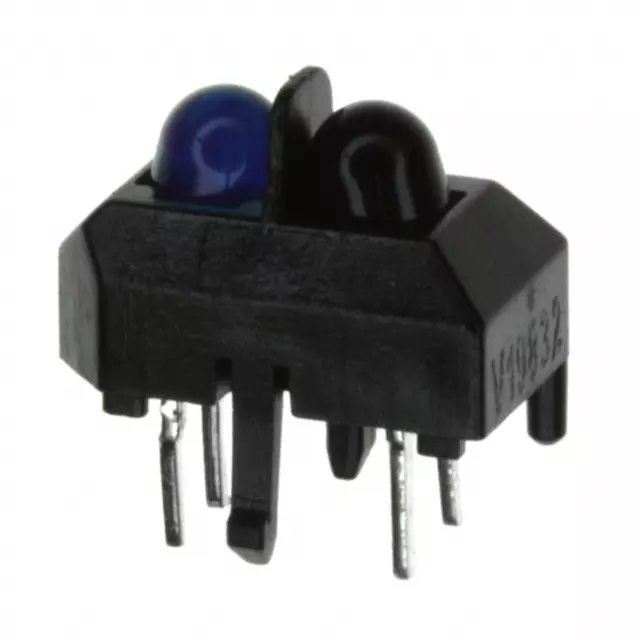
\includegraphics[height=5cm]{tcrt5000.png}
	\caption{TCRT5000 infrarood sensor\label{fig:tcrt5000}}
\end{figure}

\subsubsection*{Sensor-cel}
De TCRT5000 bestaat uit 2 belangrijke onderdelen: ten eerste hebben we een IR-led , deze led wordt aangestuurd met een voorschakelweerstand van $330\,\mathrm{\Omega}$. Ten tweede heeft de TCRT5000 een transistor die zich in essentie als infrarood-gevoelige weerstand gedraagt, samen met een serieweerstand van $68\,\mathrm{k\Omega}$ vormt dit een spanningsdeler. De IR-led zal infraroodgolven uitstralen, naargelang de ondergrond waar dit op invalt worden deze golven quasi volledig of amper gereflecteerd. Bij een witte ondergrond zal de reflectie groot zijn en de weerstand tussen collector en emittor bijgevolg zeer klein zijn, omgekeerd hebben we bij een zwarte ondergrond een grote weerstand. De uitgangsspaning bij de spanningsdeler met de weerstand en de TCRT5000-pinnen zoals u ziet in figuur~\vref{fig:tcrt5000cel} geeft dus een maat voor de reflectieco\"efficient van het oppervlak onder de sensor. De waarde van deze spanning wordt door een analoge pin ingelezen, uit deze inlezing kan dus afgeleid worden of de sensor zich boven een witte of een zwarte ondergrond bevindt. Bij een witte ondergrond bedraagt deze waarde ongeveer $30$ tot $50$ terwijl een zwarte ondergrond in een waarde tussen de $600$ en $800$ resulteert.

\begin{figure}[H]
	\centering
	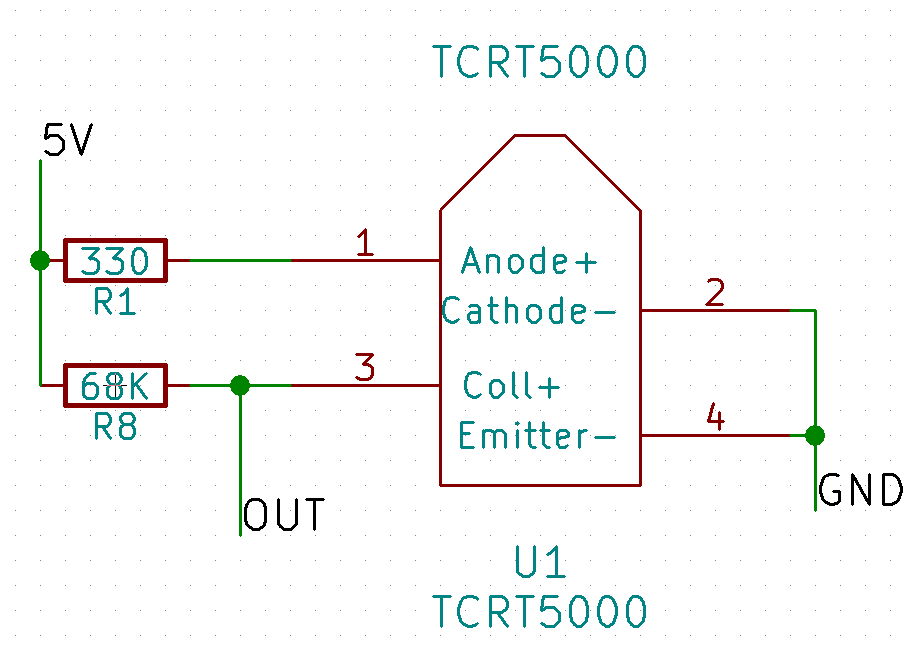
\includegraphics[height=5cm]{tcrt5000cel.png}
	\caption{Sensor-cel met TCRT 5000\label{fig:tcrt5000cel}}
\end{figure}

\subsubsection*{Sensor-arrays}
Om de positie van ons voertuig te detecteren ten opzichte van een witte zijlijn maakten we twee sensor-arrays van elk vier sensoren die via een multiplexer op een aparte printplaat ingelezen worden in \'e\'en analoge pin. De positionering van deze sensoren ziet u in figuur~\vref{fig:sensorarraypositionering}. In figuren~\vref{fig:sensorarrayvooraan} en~\vref{fig:sensorarrayachteraan} ziet u de twee verschillende sensorarrays.

\begin{figure}[H]
	\centering
	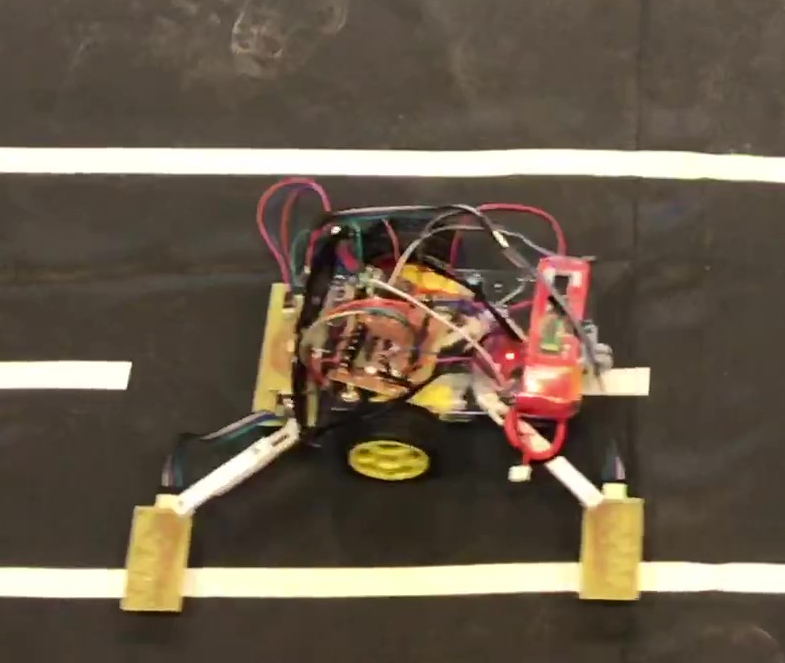
\includegraphics[height=5cm]{sensorarraypositionering.png}
	\caption{Sensorarray op het wagentje ten opzichte van de zijlijn\label{fig:sensorarraypositionering}}
\end{figure}

\begin{figure}[H]
	\centering
	\begin{minipage}[b]{0.4\textwidth}
		\centering
		\includegraphics[height=5cm]{sensorarrayvooraanonderkant.png}
		\caption{Sensorarray linksvooraan}
		\label{fig:sensorarrayvooraan}
	\end{minipage}
	\hfill
	\begin{minipage}[b]{0.4\textwidth}
		\centering
		\includegraphics[height=5cm]{sensorarrayachteraanonderkant.png}
		\caption{Sensorarray linksachteraan}
		\label{fig:sensorarrayachteraan}
	\end{minipage}
\end{figure}

\subsection{Multiplexers}
Aangezien we slechts over een beperkt aantal analoge ingangen beschikken zullen we de verschillende sensoren moeten multiplexen, hiervoor maken we gebruik van een CD4051BE-multiplexer in figuur~\vref{fig:cd4051be}, de pinout van deze IC vindt u in figuur~\vref{fig:cd4051be_pinout}. We gebruiken deze multiplexer om acht sensoren in te kunnen lezen op \'e\'en analoge pin: A0, hiervoor gebruiken we drie digitale pinnen D0,D1 en D2, die de bit selects van de multiplexer aansturen.

\begin{figure}[H]
	\centering
	\begin{minipage}[b]{0.4\textwidth}
		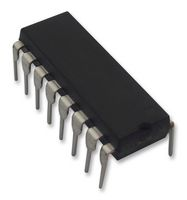
\includegraphics[height=5cm]{cd4051be.png}
		\caption{CD4051BE multiplexer}
		\label{fig:cd4051be}
	\end{minipage}
	\hfill
	\begin{minipage}[b]{0.4\textwidth}
		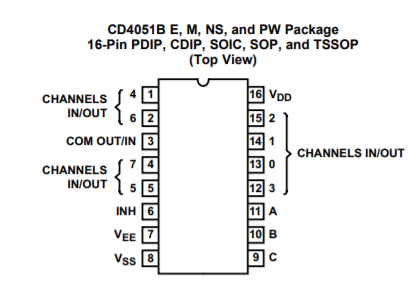
\includegraphics[height=5cm]{cd4051be_pinout.png}
		\caption{CD4051BE multiplexer pinout}
		\label{fig:cd4051be_pinout}
	\end{minipage}
\end{figure}
\subsection{Hall-sensor en magneten}\label{sec:hall-sensor}
Voor het meten van de snelheid zullen we moeten bepalen hoeveel rotaties de wielen maken gedurende een bepaalde periode. Uit dit aantal rotaties kunnen we vervolgens de afgelegde weg en dus ook de snelheid berekenen. We hebben dus een manier nodig om te detecteren wanneer en hoeveel keer het wiel een rotatie maakt, daarvoor kozen we voor het gebruik van een Hall-sensor die het passeren van magneten gemonteerd in de wielas detecteert. De gebruikte Hall-sensor is de SS41 digitale Hall-sensor van Honeywell die gevoed wordt op $5\,\mathrm{V}$. De output van deze sensor wordt aangesloten aan pin D4. In figuur ~\vref{fig:wielmagneten} ziet u de magneten die binnen in de wielas gemonteerd werden, merk op dat deze magneten een tegengestelde polarisatie hebben. In figuur~\vref{fig:hallsensor} ziet u hoe de Hall-sensor bij het wiel gemonteerd is.

\begin{figure}[H]
	\centering
	\begin{minipage}[b]{0.4\textwidth}
		\centering
		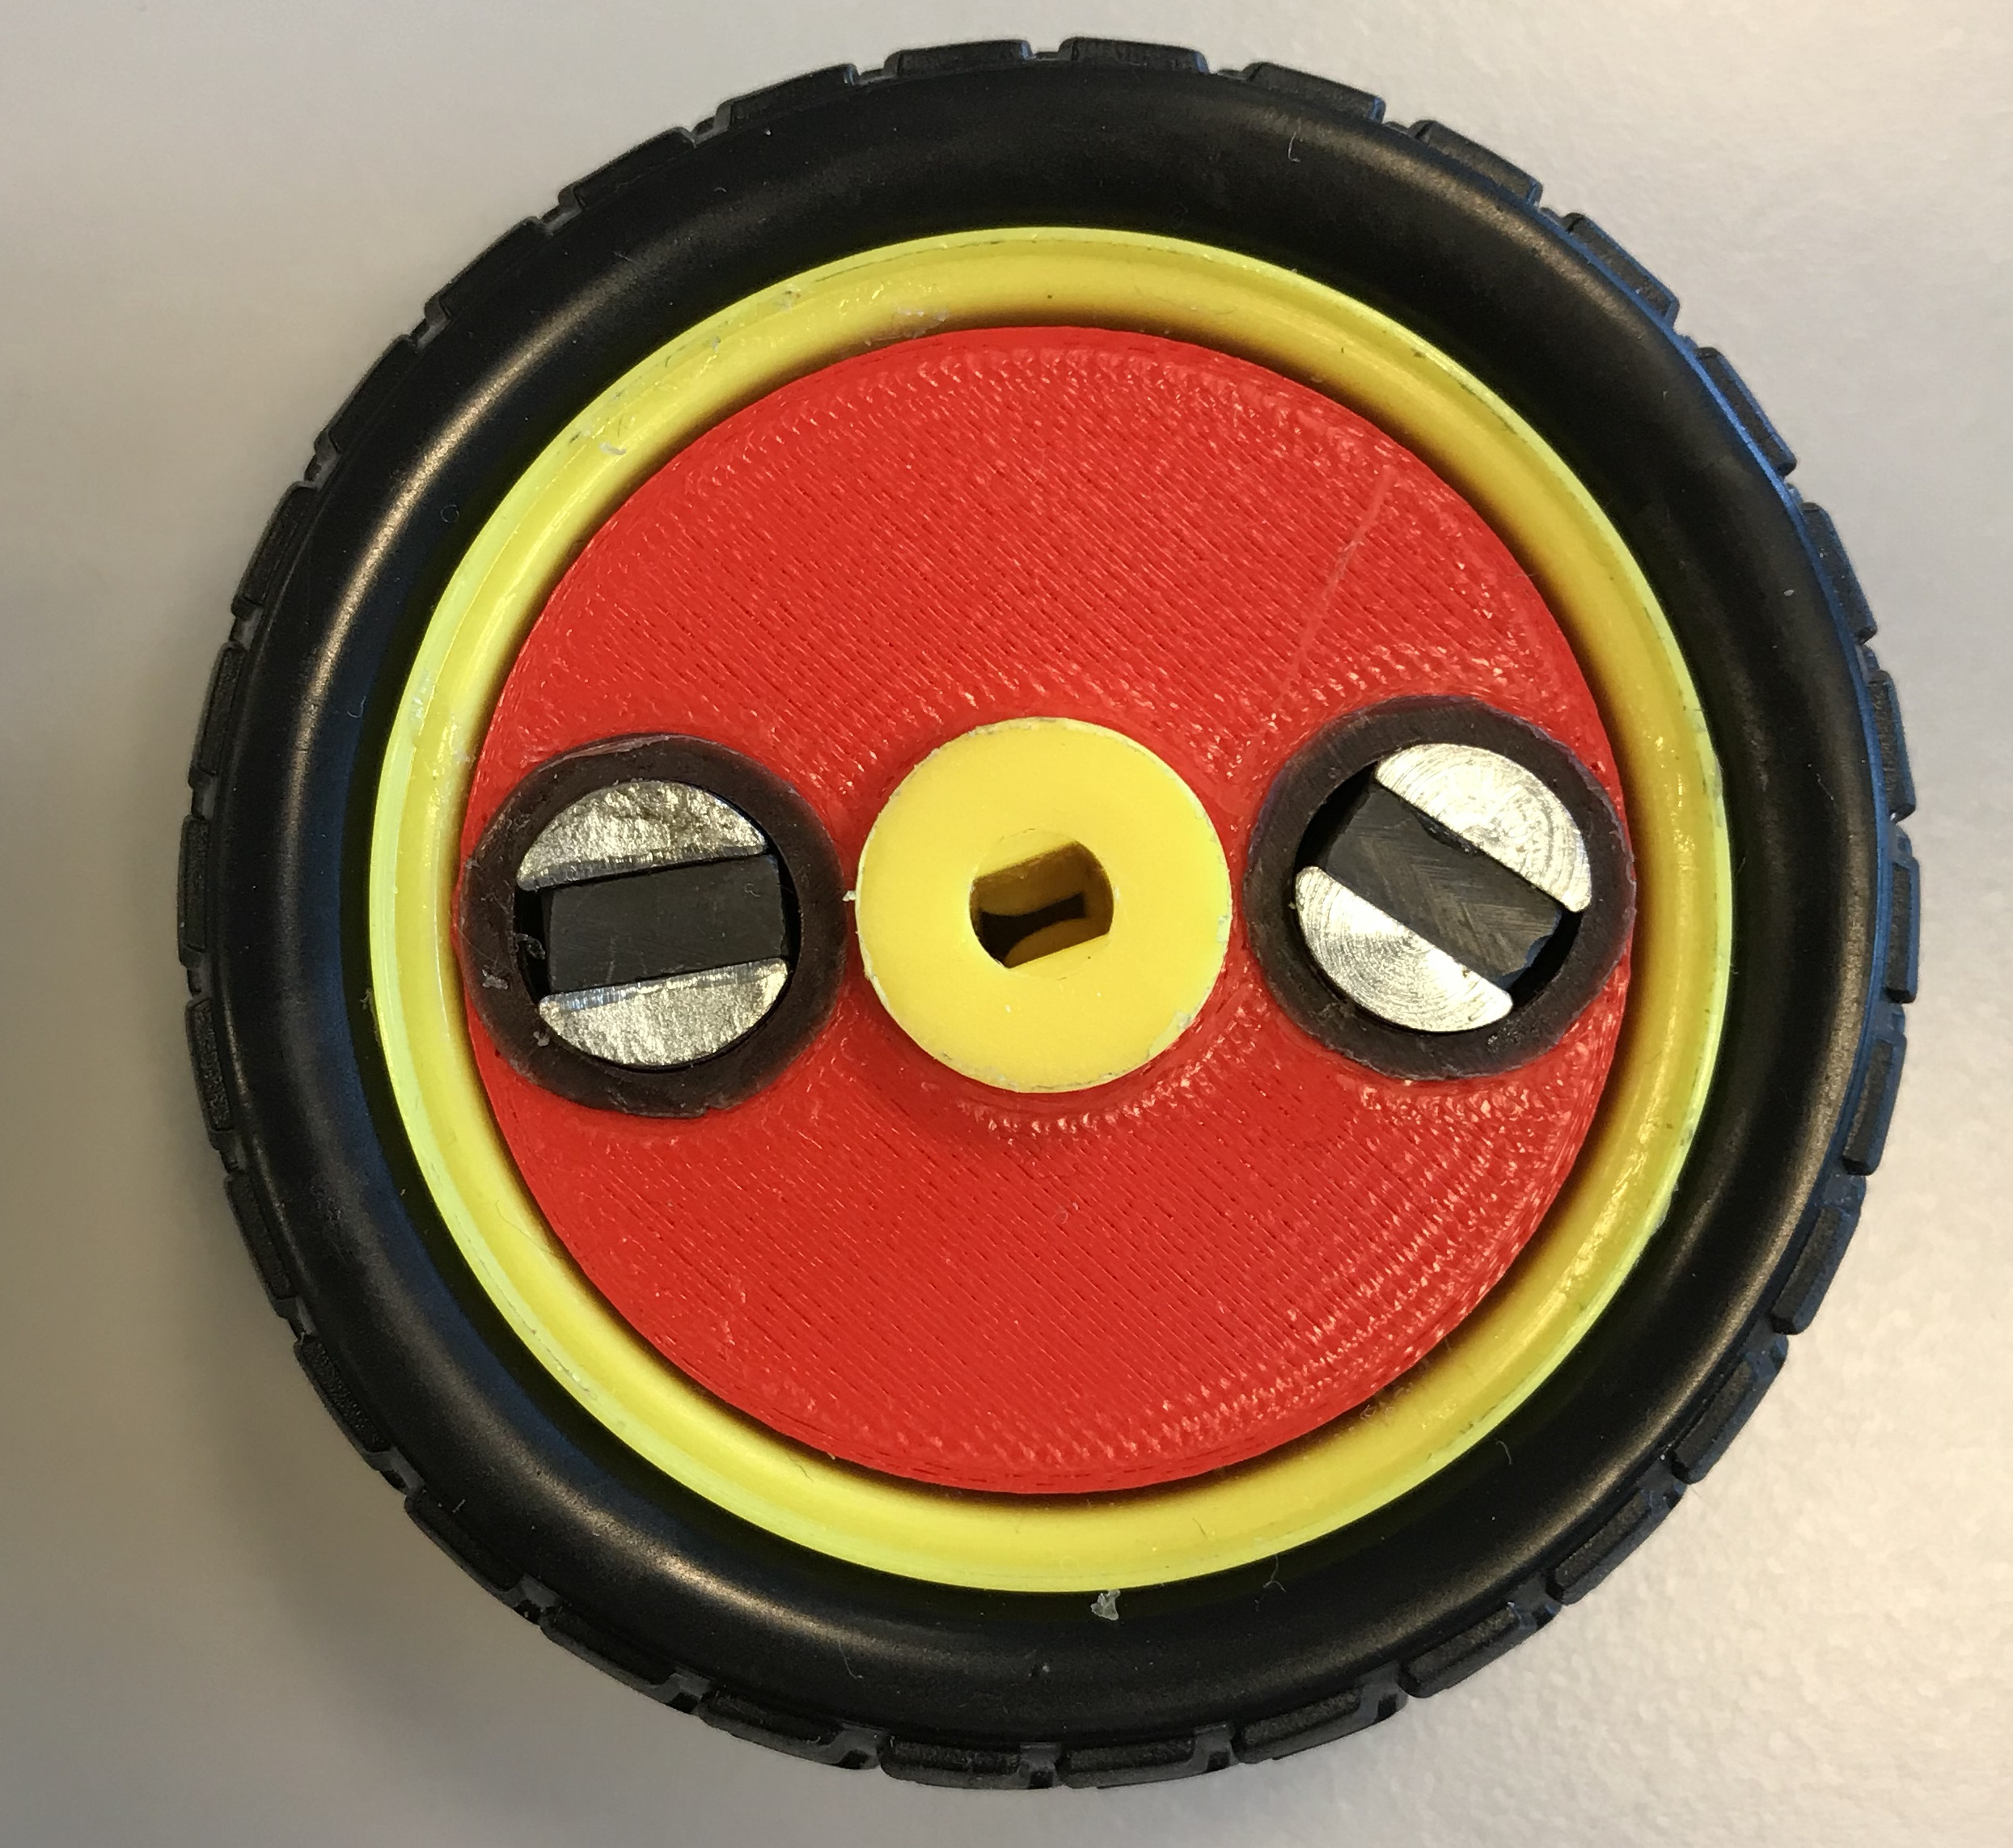
\includegraphics[height=5cm]{wielmagneten.png}
		\caption{Magneten gemonteerd in wielas\label{fig:wielmagneten}}
	\end{minipage}
	\hfill
	\begin{minipage}[b]{0.4\textwidth}
		\centering
		%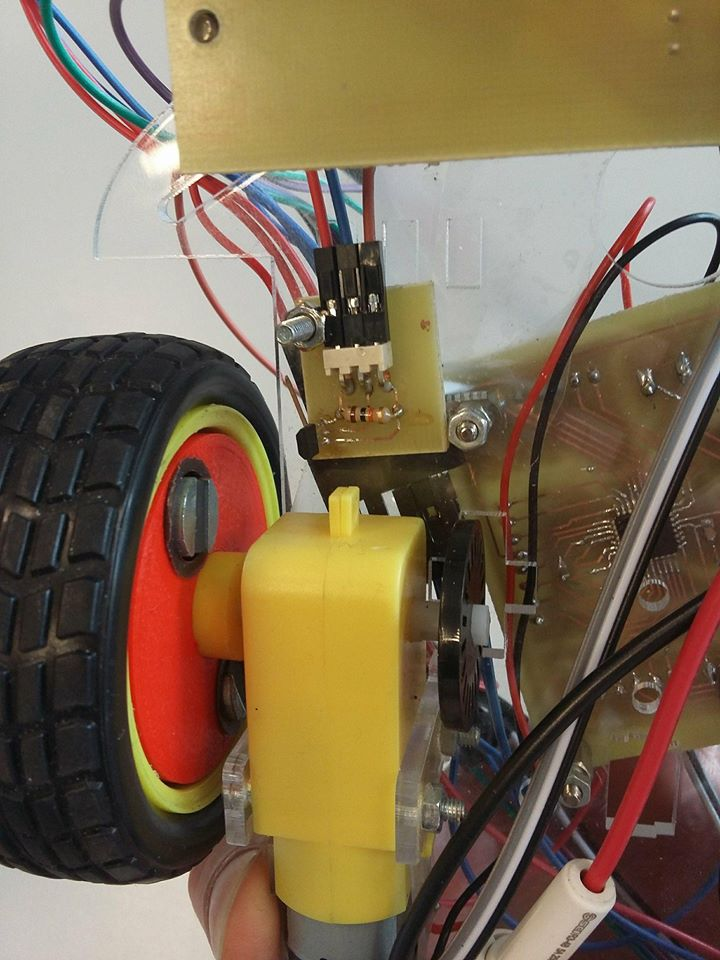
\includegraphics[height=5cm]{hallsensor.png}
		\caption{Hall-sensor gemonteerd naast wiel\label{fig:hallsensor}}
	\end{minipage}
\end{figure}

\subsection{RFID-reader}
Het inlezen van de RFID-tags gebeurt met behulp van de PN532 NFC-module v3 van Elechouse die u ziet in figuren~\ref{fig:pn532} en~\ref{fig:rfidlezermontage}. Deze module is voorzien van aansluitingen voor communicatie over HSU (High Speed UART), I\textsuperscript{2}C en SPI. De gewenste communicatie-interface wordt gekozen aan de hand van de twee SMD-switches op de module. We maken gebruik van I\textsuperscript{2}C om de tags in te lezen, de reden van deze keuze zullen we verder bespreken in hoofdstuk~\vref{sec:problemen-en-moeilijkheden}. We sluiten dus volgende pinnen van de PN532-module aan:
\begin{itemize}
	\item GND: Ground van de module, aangesloten aan de GND van onze Arduino.
	\item VCC: Voeding van de module, aangesloten aan 5\,V van onze Arduino.
	\item SDA: Seri\"ele data-pin van de module, wordt aangesloten aan pin A4 van onze Arduino.
	\item SDA: Seri\"ele clock-pin van de module, wordt aangesloten aan pin A5 van onze Arduino.
\end{itemize}

\begin{figure}[H]
	\centering
	\begin{minipage}[b]{0.4\textwidth}
		\centering
		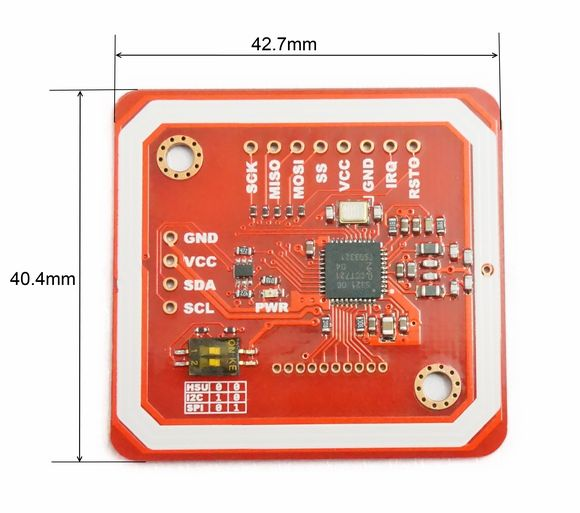
\includegraphics[height=5cm]{rfidlezer.png}
		\caption{PN532 NFC-module\label{fig:pn532}}
	\end{minipage}
	\hfill
	\begin{minipage}[b]{0.4\textwidth}
		\centering
		%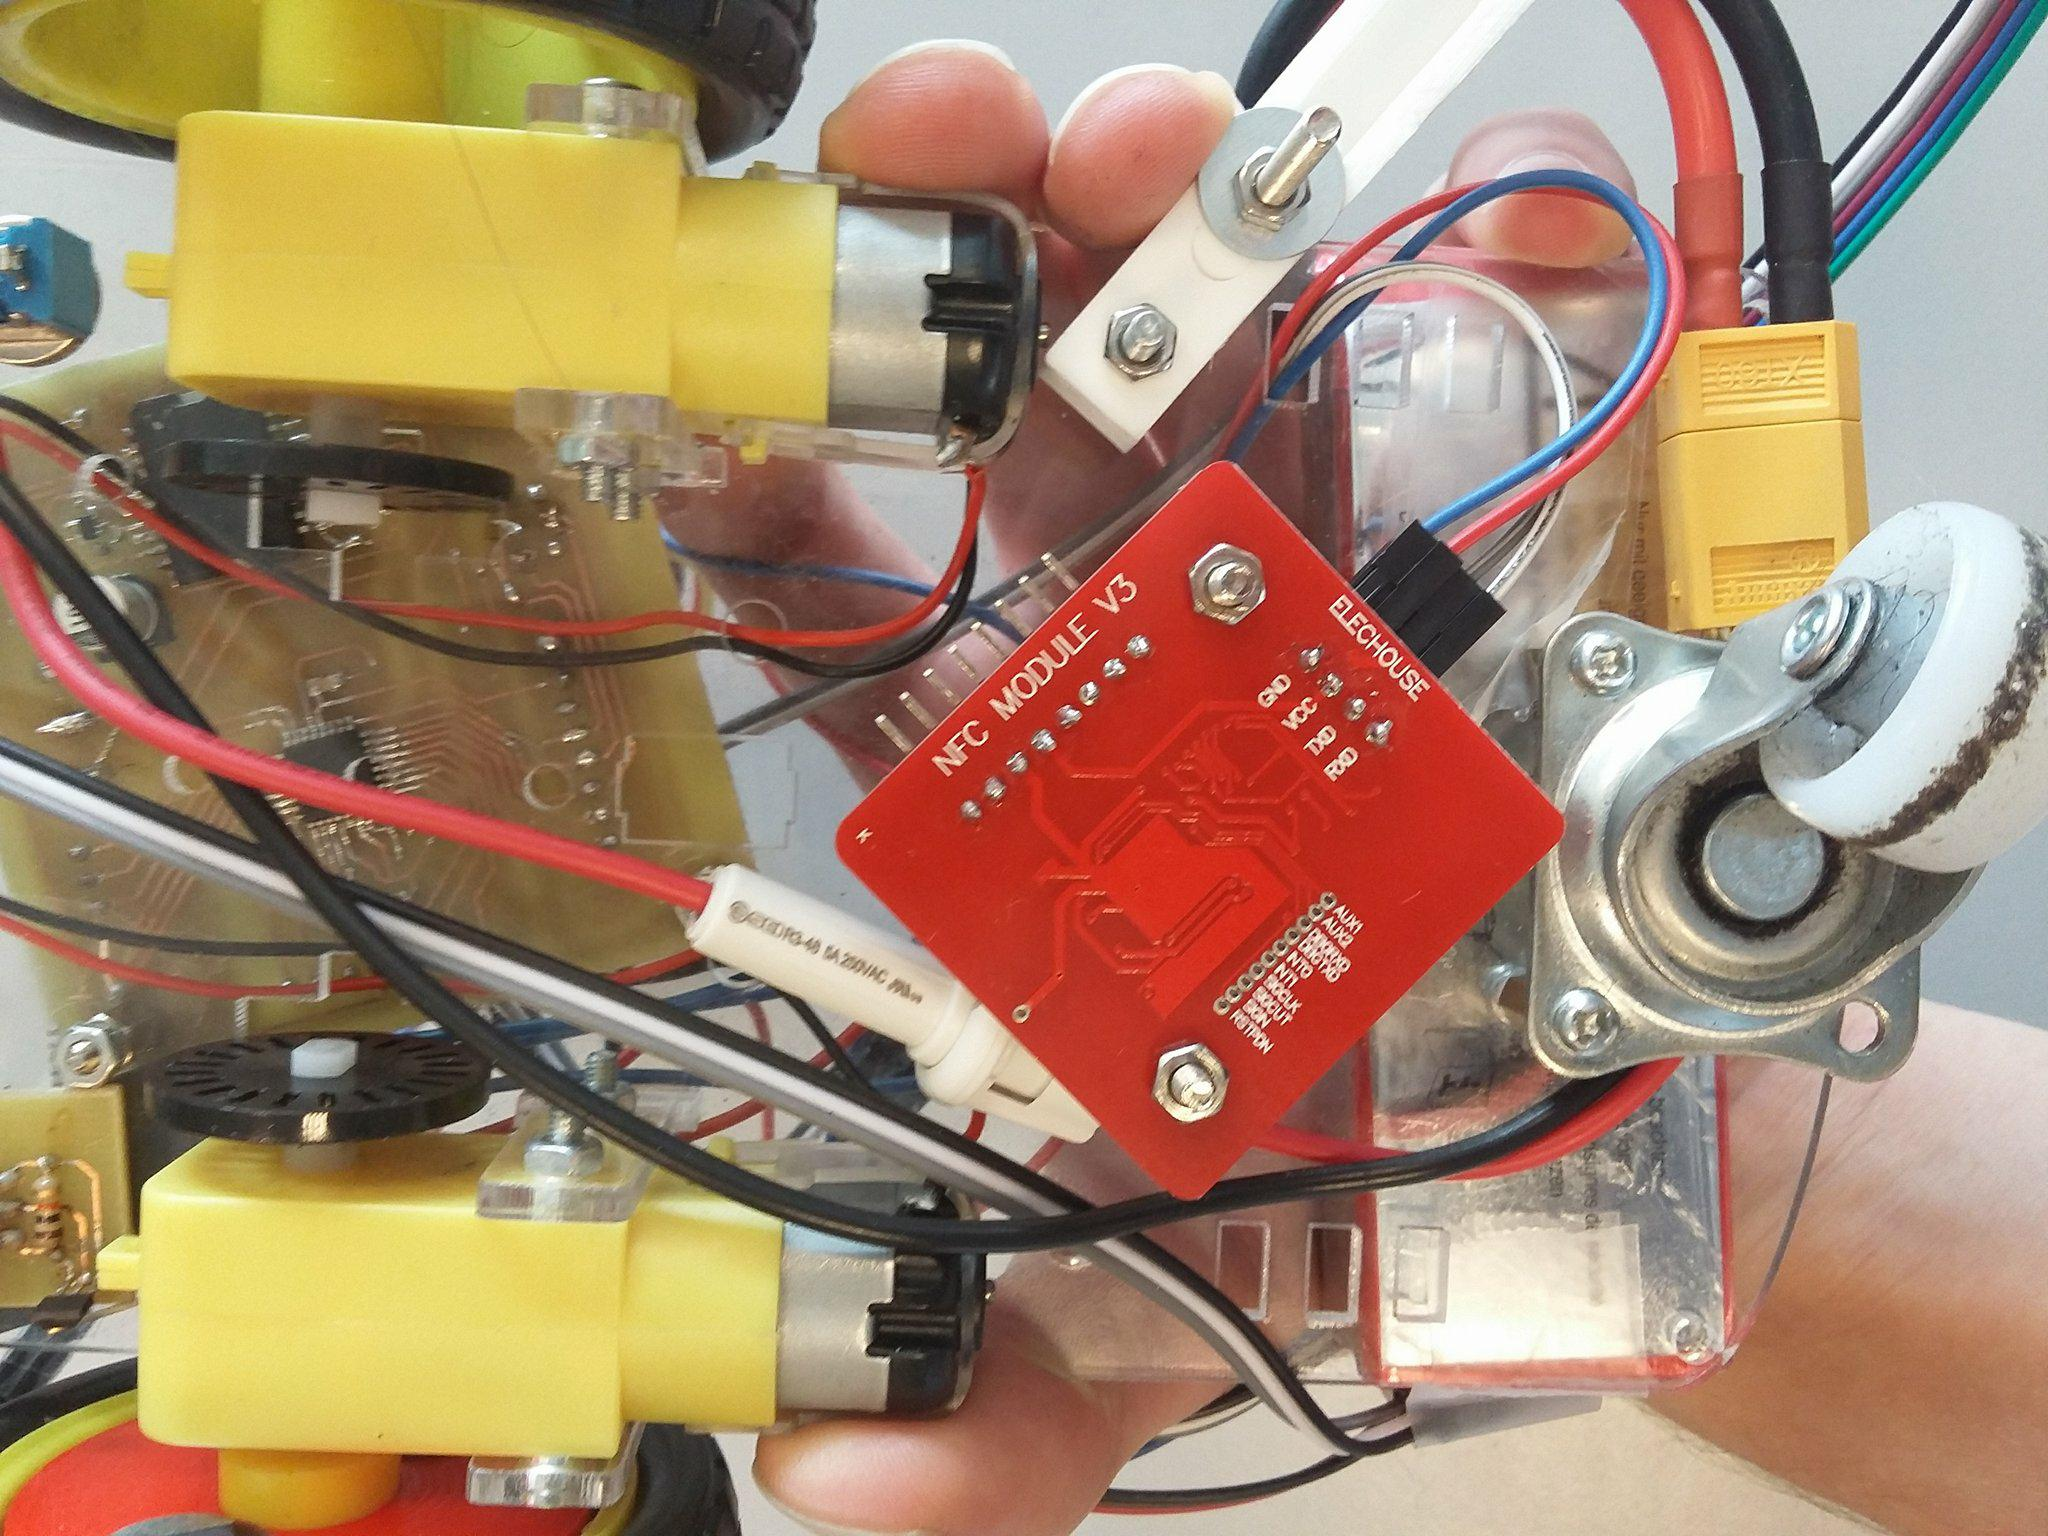
\includegraphics[height=5cm]{rfidlezermontage.png}
		\caption{PN532 op het wagentje\label{fig:rfidlezermontage}}
	\end{minipage}
\end{figure}
\subsection{Bluetooth-module}
Om Bluetooth-communicatie met een Raspberry Pi3 mogelijk te maken wordt gebruik gemaakt van de HC05 Bluetooth-module. Deze module ziet u in figuren~\ref{fig:hc05} en~\ref{fig:hc05montage}. De HC05 beschikt over zes pinnen:
\begin{itemize}
	\item EN: Dit is een enable voor de module die actief laag is, deze moet niet aangesloten worden aangezien we de module constant actief willen.
	\item VCC: Voeding van de module, aangesloten aan 5\,V van onze Arduino.
	\item GND: Ground van de module, aangesloten aan de GND van onze Arduino.
	\item TXD: Transmit-pin van de module, aangesloten aan RX van de Arduino op pin D7
	\item RXD: Receive-pin van de module, aangesloten aan TX van de Arduino op pin D8
	\item STATE: Geeft informatie over de toestand van de module, gaat hoog wanneer deze verbonden is en laag wanneer dat niet het geval is. Deze pin wordt niet gebruikt voor onze toepassing
\end{itemize}

\begin{figure}[H]
	\centering
	\begin{minipage}[b]{0.4\textwidth}
		\centering
		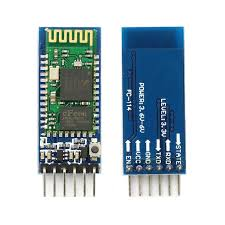
\includegraphics[height=5cm]{hc05.png}
		\caption{HC05 Bluetooth-module\label{fig:hc05}}
	\end{minipage}
	\hfill
	\begin{minipage}[b]{0.4\textwidth}
		\centering
		\includegraphics[height=5cm]{bluetoothenrfidlezer.png}
		\caption{HC05 Bluetooth-module op het wagentje\label{fig:hc05montage}}
	\end{minipage}
\end{figure}
